% Définition du nom du chapitre
\chapter[Characterisation of coralligenous reefs’ structural complexity and ecological assemblages]{Chapitre 4: Characterisation of coralligenous reefs’ \\structural complexity and ecological assemblages} \label{chapitre4-structure}

\pagestyle{main}

%%%%%%%%%%%%%%%%%%%%%%%%%%%%%
%%% Figure cover chapitre %%%
%%%%%%%%%%%%%%%%%%%%%%%%%%%%%
\begin{tikzpicture}
  \def\ig{%
   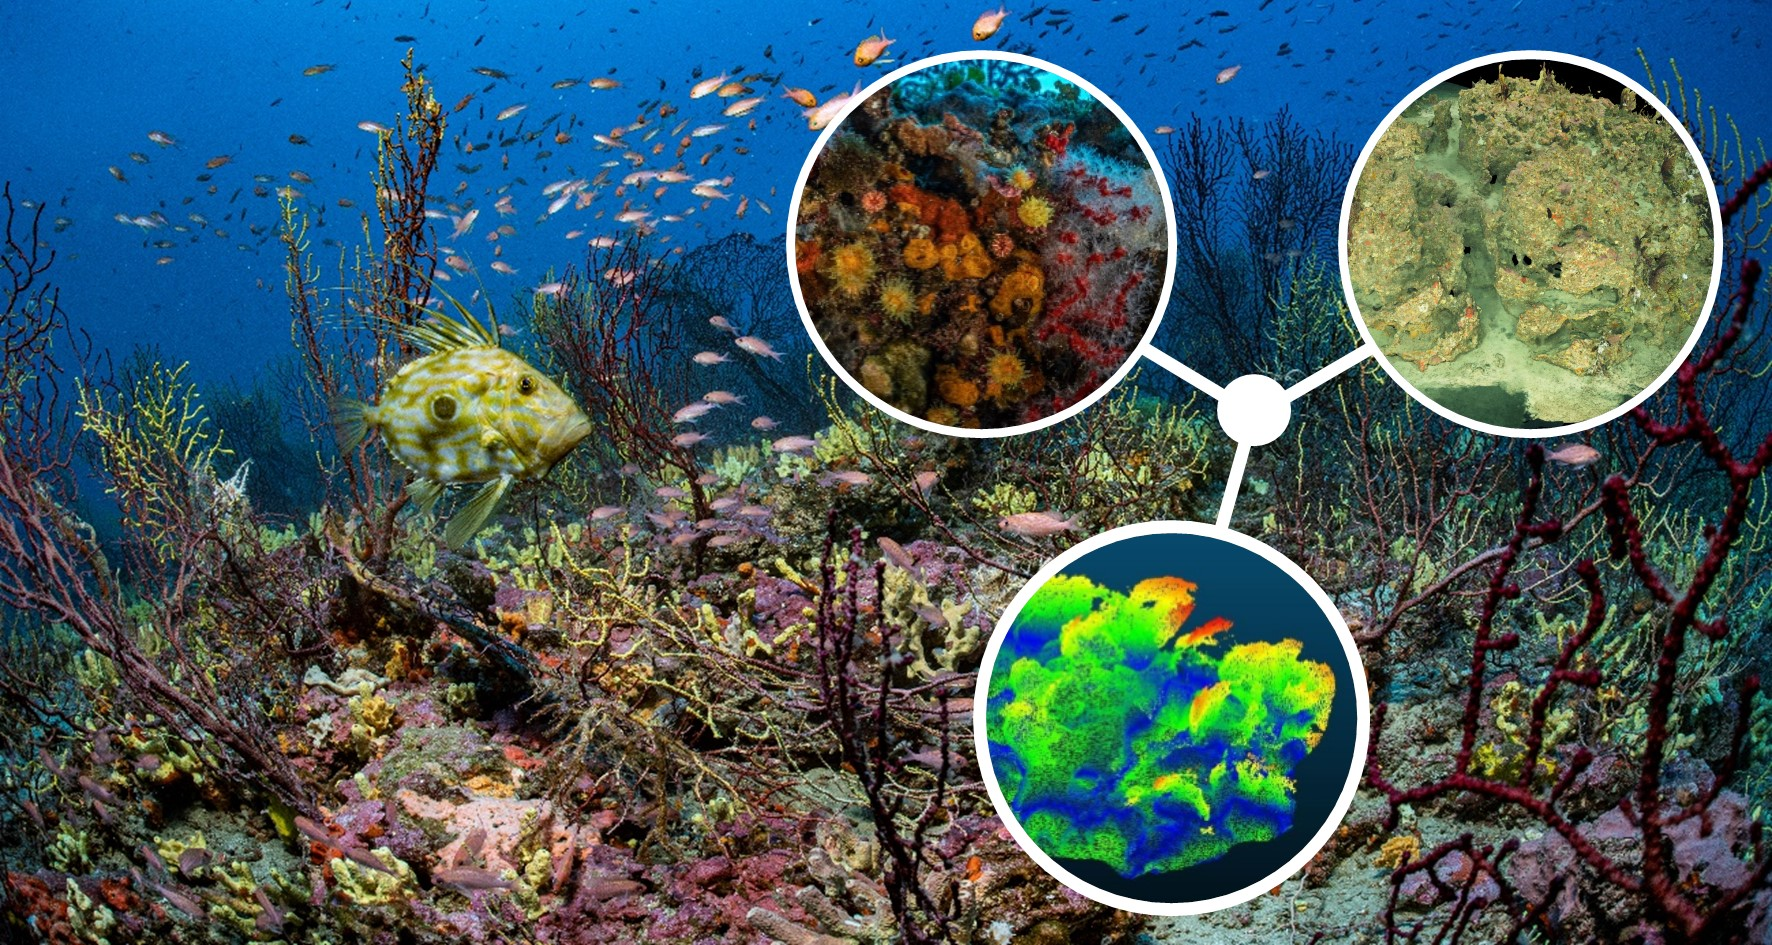
\includegraphics[width=\linewidth,keepaspectratio]{./6_chapitre4/cover_structure}}
 \node [inner sep=0pt](mypicture) at (0,0) {\phantom{\ig}};
 \clip[rounded corners=5mm] ($(mypicture.south west)+(\bord,\bord)$) rectangle ($(mypicture.north east)-(\bord,\bord)$);
 \node[inner sep=0pt](mypicture) at (0,0) {\ig};
\end{tikzpicture}


% Bullet points du début de chapitre
\setlength{\fboxsep}{8pt}
\setlength{\fboxrule}{0pt}
\begin{center}
\begin{colbox}{resume}
  \vspace{-2pt}
{\color{textresume}\small
\begin{itemize}[leftmargin=0in]\itemsep3pt
\item \textbf{OBJECTIFS}~:
    \begin{itemize}
      \item Explorer les différentes facettes de la \textbf{complexité structurale} des récifs coralligènes avec des indicateurs architecturaux~;
      \item Définir une \textbf{typologie objective} de structure des récifs basée sur ces indicateurs~;
      \item Déterminer si la \textbf{qualité écologique} et la \textbf{composition} des assemblages dépendent de la typologie structurelle~;
      \item Evaluer l'effet de l'\textbf{environnement} sur la complexité structurale~;
    \end{itemize}
\item \textbf{RESULTATS}~:
    \begin{itemize}
      \item Les \textbf{39 récifs} reconstruits par photogrammétrie se répartissent en \textbf{4 morphotypes}~;
      \item La qualité écologique et la composition des assemblages n'est \textbf{pas significativement\\ différente} entre les 4 morphotypes~;
    \end{itemize}
\end{itemize}
}
\vspace{-2pt}
\end{colbox}
\end{center}

\clearpage

\fontsize{14}{14}\noindent\textbf{Characterisation of coralligenous reefs’ structural complexity and \\ecological assemblages}

\normalsize
\medskip

% NB sans indentation
\noindent\textit{Travail exploratoire en collaboration avec Sandra Luque, Florian Holon, Pierre Boissery et Julie Deter. Encore non soumis dans une revue.}

\medskip

\noindent\textbf{Abstract}
Coralligenous reefs are considered the second richest habitat in the Mediterranean, with a biodiversity and structural complexity similar to that of coral reefs. Although the structure has been shown to play an important role in the structuration of diversity and functioning of coral reefs, no previous study accounted for the true structural complexity of coralligenous reefs measured with accurate 3D reconstruction techniques. In this study, we used 39 photogrammetric reconstructions of coralligenous reefs captured along the French Mediterranean coast to study the relationships between the 3D structure, species assemblage composition and local environmental conditions. We defined four different morphotypes based on 3D fractal dimension and rugosity indicators at different scales, from the simplest to the most complex structures. We then performed statistical analysis to assess whether environmental conditions and ecological assemblages differed across the four morphotypes. Our results did not prove any significant differences across morphotypes neither in ecological status, using both Coralligenous Assemblage Index and INDEX-COR indices, nor in assemblage composition through PERMANOVA. We asserted several hypotheses to explain these results: the much lower growth rate of coralligenous assemblages and their sheltered location in deeper waters compared to coral reefs might uncouple the observed assemblage composition from the current structure. Also, results could be affected by our species sampling procedure within the 3D reconstructed reefs, considering the high diversity and composition variability of these reefs. This study represents a first step towards the characterisation of coralligenous reefs’ structure and the relationships with the composition of assemblages, but a larger dataset and potentially a different sampling procedure are necessary to fortify or contradict our results.

\medskip

\noindent\textbf{Keywords}
benthic communities, structural complexity, photogrammetry, biodiversity, monitoring, ecological status

\newpage

\section{Introduction}\label{chapitre4_1}
Coralligenous reefs represent unique calcareous formations of biogenic origin in the Mediterranean \citep{ballesteros_mediterranean_2006}. Located at depths between 20 and 120 m below sea level, they are produced by the accumulation of encrusting algae and bioconstructor animals (polychaetes, bryozoans and gorgonians). Similar to tropical coral reefs in terms of their richness, biomass, and production \citep{bianchi_biocostruzione_2001}, coralligenous reefs are considered the second richest marine habitat in the Mediterranean Sea \citep{boudouresque_marine_2004} and described as a special habitat with biodiversity interest by the European Habitats Directive (Habitats Directive 92/43/CEE). However, these reefs are severely affected by environmental pressures, most notably increasing sediment loads and deposition coming from human coastal activities and hydrodynamics alteration \citep{airoldi_effects_2003, ballesteros_mediterranean_2006}. This habitat desperately needs to be monitored, but studying and monitoring the biodiversity of coralligenous reefs is limited by human physiological implications as it is physically demanding to spend a considerable amount of time at great depth underwater. Consequently, most  studies involve photo quadrats taken by a diver in order for the coralligenous assemblages to be identified back on land by a taxonomist \citep{deter_rapid_2012, kipson_rapid_2011, sartoretto_integrated_2017}, and derive biodiversity and conservation indices such as the Coralligenous Assemblage Index (CAI) \citep{deter_preliminary_2012} or INDEX-COR \citep{sartoretto_integrated_2017}.

Although the European Directive for the conservation of the marine realm (Directive 2008/56/\\CE) states that the good ecological status of a habitat includes the integrity of its structure, this compartment is rarely assessed. However, many studies pointed out the habitat structural complexity as one of the most important drivers structuring biological communities, notably linking increases in habitat complexity with increases in diversity and abundance of both sessile and mobile organisms \citep{darling_relationships_2017, graham_importance_2013, gratwicke_relationship_2005, harborne_biotic_2011, kovalenko_habitat_2012, luckhurst_analysis_1978, meager_topographic_2011, rees_abiotic_2014}. Conversely, the loss of structural complexity is associated to ecosystem decline in biodiversity and therefore resilience \citep{ferrari_quantifying_2016}. In the case of coral reefs, structural complexity is notably a key driver determining whether a reef stays in a coral-dominated or shifts to an algal-dominated state after a disturbance such as a storm damage or a coral bleaching event \citep{graham_predicting_2015}. Among the different structural complexity indicators used in the literature, fractal dimension was shown to be a good measure of coral reef complexity and is invariant to changes in orientation (Fukunaga et al., 2019).

Some studies have linked the very high biodiversity of coralligenous reefs to their structural complexity, known to be one of the highest in the Mediterranean Sea \citep{bianchi_biocostruzione_2001}, and to the heterogeneity of environmental conditions that create multiple habitat niches \citep{johnson_area-independent_2003, kipson_rapid_2011, willis_habitat_2005}. However, to the best of our knowledge, the only studies that considered coralligenous reefs’ structural complexity derived structural metrics from assemblages composition using a theoretical size for each species \citep{sartoretto_integrated_2017, valisano_characterization_2019}. Exploring the links between the true structure of these very slow growth reefs (0.006 – 0.83 mm.y-1 \citep{sartoretto_age_1996}) and the composition of the corresponding coralligenous assemblages requires the use of a precise 3D reconstruction technique such as photogrammetry or high resolution echo-sounder.

Underwater photogrammetry has been extensively used since the mid-2010s for the study of marine habitats, notably coral reefs’ structural complexity \citep{bryson_characterization_2017, burns_integrating_2015, burns_utilizing_2015, figueira_accuracy_2015, gutierrez-heredia_simple_2015, leon_measuring_2015}. This technique allows the reconstruction in three dimensions (3D) of an object or a scene using numerous images taken from different perspectives \citep{figueira_accuracy_2015}. Although photogrammetry tends to underestimate surface roughness for all coral morphologies \citep{figueira_accuracy_2015}, it has been proven accurate and precise for the 3D reconstruction of benthic habitats \citep{bryson_characterization_2017, figueira_accuracy_2015, marre_monitoring_2019}. With applications from the individual \citep{zawada_quantifying_2019} to the reef scale  \citep{figueira_accuracy_2015}, photogrammetry helped prove significant differences in morphology and structural complexity among coral benthic features \citep{burns_integrating_2015}. To the best of our knowledge, in the case of coralligenous assemblages, photogrammetry has only be used to quantify individual growth or count individuals so far \citep{palma_sfm-based_2018,palma_effective_2019,royer_photogrammetric_2018}. This study sought to characterise coralligenous reefs’ structural complexity using underwater photogrammetry and explore the relationships with the composition of the corresponding assemblages and the environmental conditions. We used photogrammetric and ecological data from 39 study sites to explore and draw relationships between those different compartments. More specifically, we performed the following analyses:

\begin{enumerate}
    \item Explore the different facets of coralligenous reefs’ structural complexity using metrics derived from photogrammetric models;
    
    \item Define objective reef morphotypes based on these structural metrics;
    
    \item Explore whether or not the structure determines the nature of the corresponding coralligenous species assemblages;
    
    \item Explore whether or not local environmental conditions influence the structure.
\end{enumerate}

\section{Materials and methods}\label{chapitre4_2}

\subsection{Study sites}\label{chapitre4_2.1}
The data were collected in June 2018 and 2019 for 39 study sites (\autoref{figure4.1}) located between 17 and 77 m deep along the French Mediterranean coast during the RECOR monitoring network campaigns \citep{andromede-oceanologie_recor_2020}. RECOR is the largest French initiative for the monitoring of coralligenous reefs’ ecological status along the French Mediterranean coast, from Spain to Italy, including the Corsican coast. The network includes collection of data about gorgonians density, photographic quadrats to identify the species assemblages and photogrammetric data to characterise the 3D structure of the coralligenous reefs. These data are collected and analysed in order to assess the ecological status and diversity of the reefs, investigate the correlations with environmental conditions and anthropogenic pressures to support decision makers build wise conservation policies.

%%%%%%%%%%%%%%%%%%%%%%%%%%%%%
%%% Figure 1: Study sites %%%
%%%%%%%%%%%%%%%%%%%%%%%%%%%%%
\begin{figure}[H]
	\begin{center}
	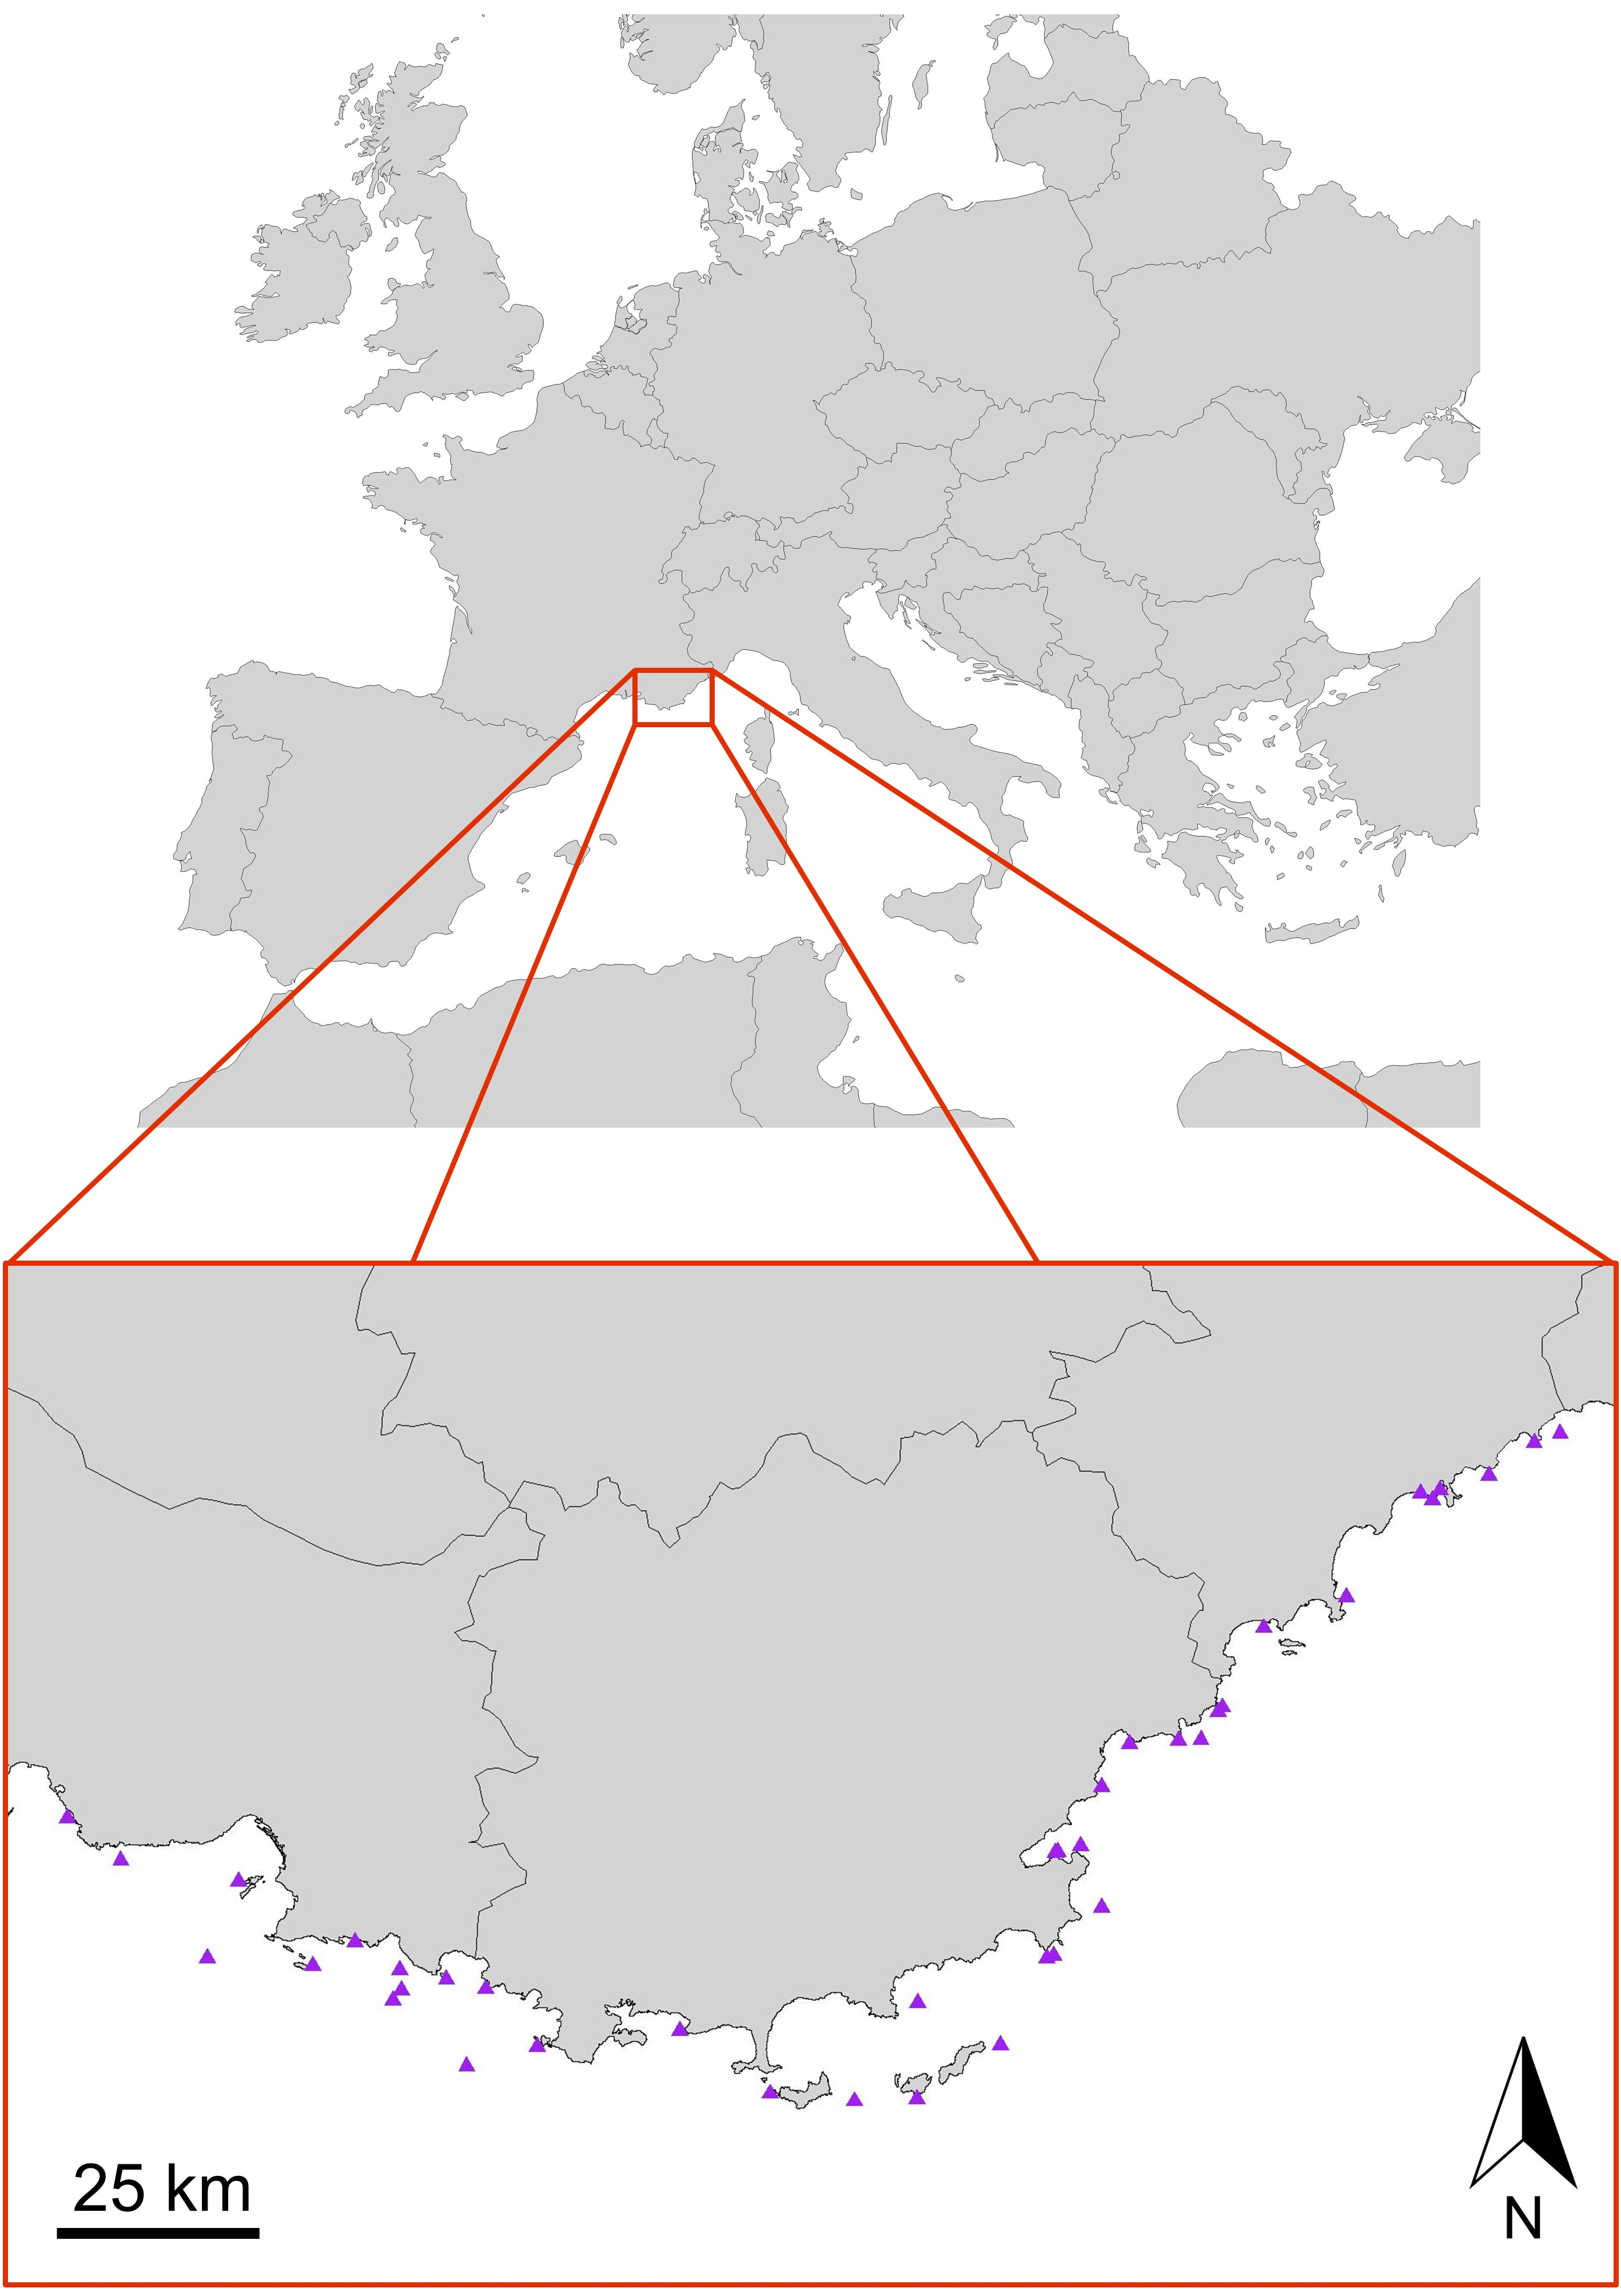
\includegraphics[width=0.7\linewidth,keepaspectratio]{./6_chapitre4/Figure4.1}
		\caption[Localisation of the 39 study sites along the French Mediterranean coast]{Localisation of the 39 study sites along the French Mediterranean coast.}
	\label{figure4.1}
\end{center}
\end{figure}

\newpage

\subsection{Structural data}\label{chapitre4_2.2}

\subsubsection{Photogrammetric acquisition and processing}\label{chapitre4_2.1.1}
All acquisitions were conducted by one scuba diver using a 16 Mega Pixel Nikon D4 in a waterproof Seacam housing, mounted with a Nikon RS 20 - 35 mm lens (set to 20 mm). For each acquisition, the diver glided around the reef at a distance of about 1.5 m, conducting parallel, regularly spaced transects at a relatively low speed of 20 - 25 m.min-1, with a time lapse of 1 s between pictures \citep{marre_monitoring_2019}. To achieve a sufficient balance between depth of field, sharpness, and exposure, camera settings were adjusted from site-to-site in accordance with the local environmental conditions (light conditions were highly variable from site to site) but high shutter speed was used in order to avoid image blurring (20 mm focal length, F11 - 13, 1 / 250 s, ISO 1250 - 3200). Focus was set automatically at the beginning of each acquisition, then turned to manual.
All datasets were processed with Agisoft PhotoScan Professional Edition V. 1.4.0 (Agisoft LLC, 2018). This commercial software is commonly used by the scientific community \citep{burns_assessing_2016, casella_mapping_2017, figueira_accuracy_2015, guo_accuracy_2016, mizuno_simple_2017} and uses a classic photogrammetric workflow. We used the self-calibration procedure implemented in PhotoScan, as the refraction effects at the air-port and port-water interfaces can be absorbed by the physical camera calibration parameters during self-calibration \citep{shortis_calibration_2015}.

Parametrisation of the different steps was set as follows: 
\begin{itemize}
    \item \textbf{Bundle adjustment:} high quality (original image resolution); key point limit = 60000 (maximum number of feature points detected on every image); no tie point limit (no upper limit for the number of associated tie points between images); generic preselection enabled (first pass using lower accuracy setting prior to the high quality adjustment, to save processing time);
    
    \item \textbf{Optimisation} (adjustment of estimated point coordinates and camera parameters minimizing the sum of reprojection error): $f$ (focal length), $cx$ – $cy$ (principal point offset), $b1$ – $b2$ (affinity and non-orthogonality coefficients), $k1$ – $k2$ – $k3$ – $k4$ (radial distortion coefficients) and p1-p2 (tangential distortion coefficients);
    
    \item \textbf{Dense cloud}: medium quality (original image resolution downscaled by a factor 4);
    
    \item \textbf{Mesh}: high quality (original image resolution) / surface type = arbitrary (any kind of object).
\end{itemize}

The models were orientated and scaled using four coded markers fixed on a 0.9 $\times$ 0.9 m cross-scale bar, located nearby each reef. All meshes were manually cleaned in order to remove the edges and gross artefacts visible on the scenes.

\subsubsection{Structural complexity measurements}\label{chapitre4_2.1.2}
All meshes were sampled using the mesh sampling tool implemented in CloudCompare Version 2.10 (CloudCompare, GPL software, 2018), with a point density of 10 000 points / m² (corresponding to 1 point / cm²). Structural complexity measurements were computed as follows:

\begin{itemize}
    \item \textbf{Roughness index} for all points of all sampled point clouds using CloudCompare, with different kernel sizes: 0.02, 0.05, 0.1, 0.15, 0.2, 0.3, 0.4, 0.5, 0.75, 1.0 m (\autoref{figure4.2});
    
    \item \textbf{Fractal dimension} (D) of each point cloud using an R \citep{r_core_team_r_2020} custom counting box algorithm \citep{liebovitch_fast_1989}.
    
\end{itemize}

%%%%%%%%%%%%%%%%%%%%%%%%%%%%%
%%% Figure 2: Study sites %%%
%%%%%%%%%%%%%%%%%%%%%%%%%%%%%
\begin{figure}[H]
	\begin{center}
	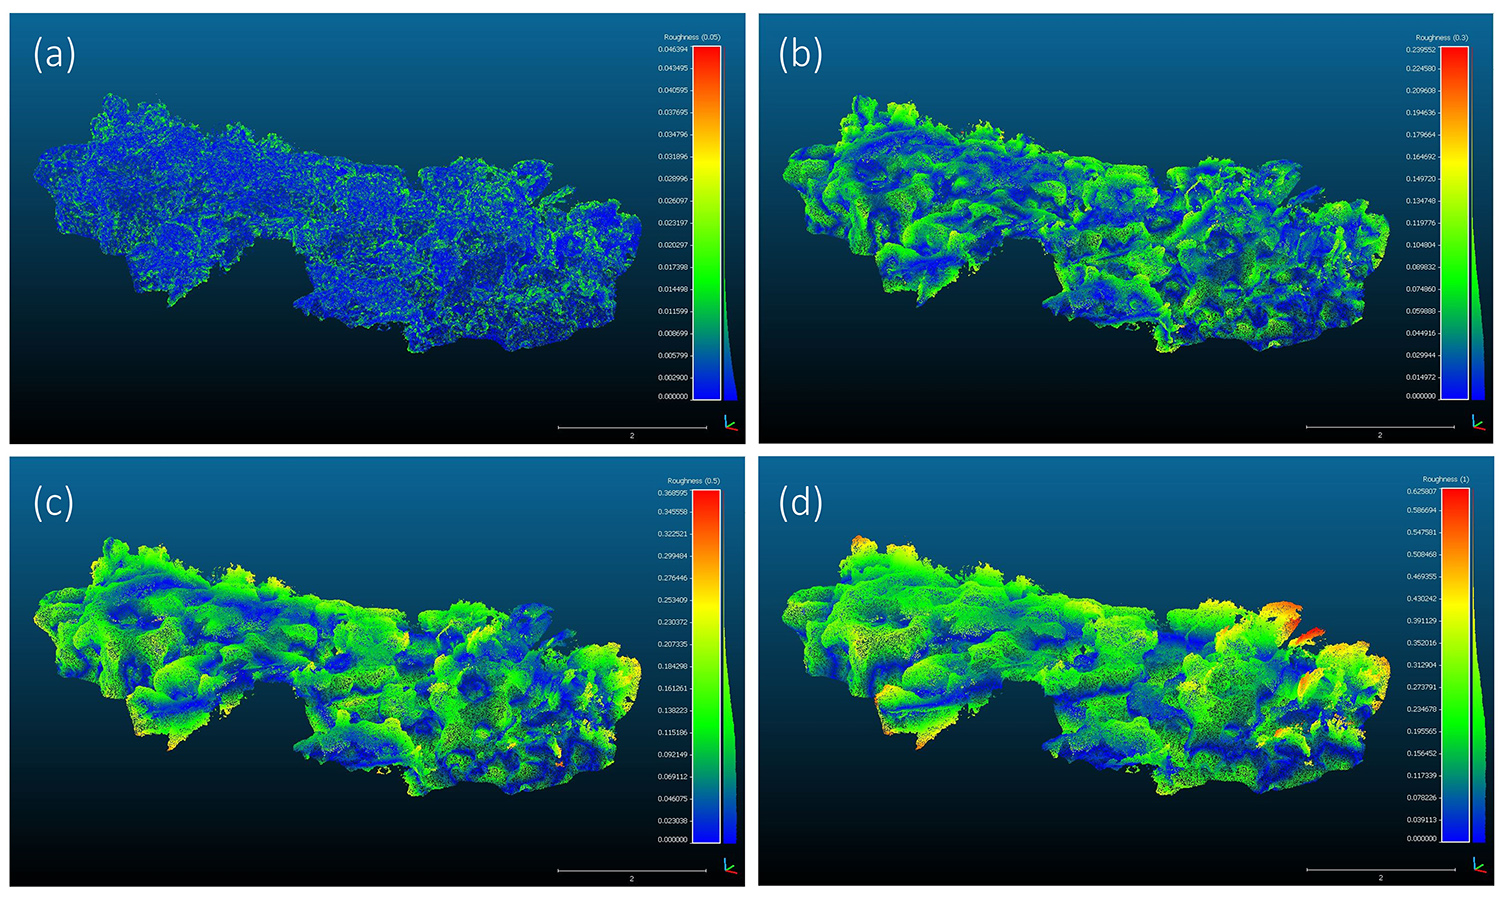
\includegraphics[width=\linewidth,keepaspectratio]{./6_chapitre4/Figure4.2}
		\caption[Roughness of site “Mimosa” with different kernel sizes]{Roughness of site “Mimosa” with different kernel sizes: (a) 0.05 m, (b) 0.3 m, (c) 0.5 m, (d) 1 m.}
	\label{figure4.2}
\end{center}
\end{figure}

\newpage

\subsection{Ecological data}\label{chapitre4_2.3}
All photographic quadrats were acquired by one scuba diver, using a Nikon D810 camera in a waterproof Seacam housing, fitted with two lateral strobes, fixed on a quadrat frame for standard acquisition (2 500 cm² quadrat). The resolution was 36.3 megapixels (Mpx), and the focal length 20 mm. Camera settings were adjusted from site to site, depending upon the local environmental conditions and reef morphology, in order to achieve a sufficient balance between depth of field, sharpness, and exposure (F16, 1 / 200 s, ISO 100 - 400). The shutter speed was consistently set to high in order to avoid image blurring (1 / 200 s) and the focus was set automatically at the beginning of each acquisition, then set to manual. Thirty quadrats were analysed per station onto which 64 points were randomly projected and manually labelled by the same taxonomist using the Coral Point Count v4.1 “coralligenous assemblages version” \citep{cpce_coral_2011} software \citep{deter_rapid_2012}.

All projected points on the quadrats were labelled at different taxonomic levels (species, gender, phylum; hereafter called “classes”) as all species cannot be distinguished with only visual aspect and can require morphological and/or genetic analyses. This corresponded to 74 880 labelled points (39 sites $\times$ 30 quadrats $\times$ 64 random points) and 124 different classes from 12 different major categories: ascidians, brown macroalgae, encrusting bryozoans, encrusting red macroalgae, erected bryozoans, erected red macroalgae, gorgonians, green macroalgae, hydroid, scleractinians, sponges and substrate (sand, pavement, rubble, sludge). An extra label, hereafter mentioned as cavity, corresponded to dark blue parts of the quadrats because of the depth in the image. 

Several indicators accounting for different facets of biodiversity and coralligenous ecological status were computed for each study site, based on the identifications on the photo quadrats:
\begin{itemize}
    \item \textbf{Taxonomic Diversity (TD)}: number of different classes observed on a given site;
    
    \item \textbf{Shannon Index (SI):} takes abundance into account in order to attribute more or less weight to common or rare classes \citep{magurran_measuring_2004}:
    
    \begin{equation}
	S_j=-\sum_{i}p_{ij} log(p_{ij})
	\label{eq4.1}
    \end{equation}

    With \textit{p\textsubscript{ij}} the prevalence of species \textit{i} among site \textit{j}.

    \item \textbf{Functional Diversity (FD)}: facet of biodiversity that quantifies the value and range of organismal traits influencing their performance and by extension, ecosystem functioning \citep{diaz_vive_2001}. We used a functional dendrogram-based index to compute FD \citep{mouchet_towards_2008} based on a trait database compiled by \citet{doxa_mapping_2016}. This database included a large set of traits to avoid the risk of over-estimating functional redundancy \citep{calba_measuring_2014}. Classes that corresponded to a coarser taxonomic level than the species level were discarded from functional analyses;
    
    \item \textbf{Coralligenous Assemblage Index (CAI)} \citep{deter_preliminary_2012}: assessment of the coralligenous ecological status based on the prevalence of bryozoans, major builders and sludge in an assemblage :
    \begin{equation}
    \text{CAI\textsubscript{i}}=\frac{1}{3}\times(\frac{1-sludge_i}{1-\min_{i}sludge_i}+\frac{majbuilders_i}{\max_{i}majbuilders_i}+\frac{bryozoans_i}{\max_{i}bryozoans_i})
    \label{eq4.2}
    \end{equation}

    With \textit{sludge\textsubscript{i}}, \textit{majbuilders\textsubscript{i}} and \textit{bryozoans\textsubscript{i}}, the covering percentage of sludge, major builders and bryozoans in site $i$.
    
    \item \textbf{INDEX-COR (IC)} \citep{sartoretto_integrated_2017}: assessment of the coralligenous ecological status based on the number of observed species, the sensitivity to organic matter and sediment loads, and structural complexity to some extent. IC was calculated as follows:
    
    \begin{equation}
    \text{IC}=0.62\times TS + 0.6\times OTR + 1.7\times SC
    \label{eq4.3}
    \end{equation}

    With TS = Taxa Sensitivity: sensitivity of the assemblage to organic matter and sediment input; OTR = Observable Taxonomic Richness: same as Taxonomic Diversity; SC = Structural Complexity: stratified structure of coralligenous habitats (see \citet{sartoretto_integrated_2017} for more details on the methodology).
    
\end{itemize}


\subsection{Environmental conditions}\label{chapitre4_2.4}
In order to explore the links between the morphotypes and the ecology of coralligenous reefs, we accounted for several environmental variables that could influence the structure and composition of assemblages. More particularly, we accounted for: sea bottom temperature, salinity, suspended matter and horizontal current data were downloaded from Previmer predictions (MARS3D v10.10 model \citep{ifremer_mars_2019}) over the period 2015-01 until 2019-11, with one observation per week over the whole Western Mediterranean. For each variable, data was extracted from original raster layers at the geographical locations of the 39 study sites at the bottom depth, and the mean over the whole period was used as a predictor for further analysis. Depth was also used as an environmental variable.

\subsection{Data analysis}\label{chapitre4_2.5}

\subsubsection{From structural descriptors to morphotypes }\label{chapitre4_2.5.1}
For the different kernel sizes, we computed the mean, standard deviation and quantiles ($Q_{10}$, $Q_{25}$, $Q_{50}$, $Q_{75}$ and $Q_{90}$) of roughness across all points for each study site. For each kernel size, we removed all highly correlated variables (spearman correlation coefficient > 0.7) and we performed a Principal Component Analysis (PCA) on all the roughness descriptors (all kernel sizes together) along with the fractal dimension. Principal components were then used to cluster sites by morphotype. The number of components was defined as the minimum number of components necessary to capture 90 \% of the variance in the data. Morphotypes were defined using K-means clustering (R package ClusterR v1.2.1) with K = 4 clusters. Considering the relatively low amount of observations (39 study sites), we used spearman correlation coefficient and Linear Models (LM) to assess the links between structural variables. Each LM was initially built with all corresponding predictors, then pruned by dropping the least significant predictor until all remaining predictors were significant.

\subsubsection{Quantifying the relationships between morphotypes, coralligenous assemblages and environmental conditions }\label{chapitre4_2.5.2}
Considering biodiversity indicators, ecological status indices and environmental variables, the normality of distributions and equality of variances across the four morphotypes were tested using Shapiro-Wilkinson and F-test, respectively. If a variable did satisfy both conditions, we compared the means between morphotypes two-by-two using t-tests; otherwise, we used non-parametric Mann-Whitney-Wilcoxon (MWW) tests. Abundance data were analysed with permutational multivariate analysis of variance PERMANOVA \citep{anderson_new_2001} under unrestricted permutation of the raw data (9999 permutations) to test the response of assemblage composition to the morphotype. Additionally, a non-metric multidimensional scaling (nMDS) \citep{clarke_primer_2006} was used as ordination plot to visualise the convex hull of each morphotype on a 2D space. All analyses and calculations were performed with R Software v3.6.3 \citep{r_core_team_r_2020}. Ecological analyses used vegan R package v2.5.6.

\section{Results}\label{chapitre4_3}

\subsection{Study sites’ structural complexity}\label{chapitre4_3.1}
For all kernel sizes, all roughness statistical descriptors were highly correlated (spearman correlation coefficient > 0.8). Consequently, only the mean of each kernel size was kept for further analysis. F ranged between 2.02 and 2.20 across the 39 study sites, and was moderately correlated to mean roughness with kernels 0.15, 0.20 and 0.30 m (spearman correlation coefficient 0.62 – 0.65). The means of roughness with kernel sizes 0.05 and 0.5 m significantly contributed to explain the fractal dimension (t-test; p-value < 0.01 and 0.001, respectively) with 39 \% of explained variance.

The three first axes of the PCA on roughness means and fractal dimension accounted for 93 \% of the total variance. The K-means clustering defined four different clusters, hereafter called “morphotypes”: morphotype 1 corresponded to low complexity sites (6 sites), morphotype 2 to average complexity with small structures (15 sites), morphotype 3 to average complexity with large structures (13 sites) and morphotype 4 to high complexity with large structures (5 sites; \autoref{figure4.3}).

%%%%%%%%%%%%%%%%%%%%%%%%%%%%%
%%% Figure 3: Biplot PCA %%%
%%%%%%%%%%%%%%%%%%%%%%%%%%%%%
\begin{figure}[H]
	\begin{center}
	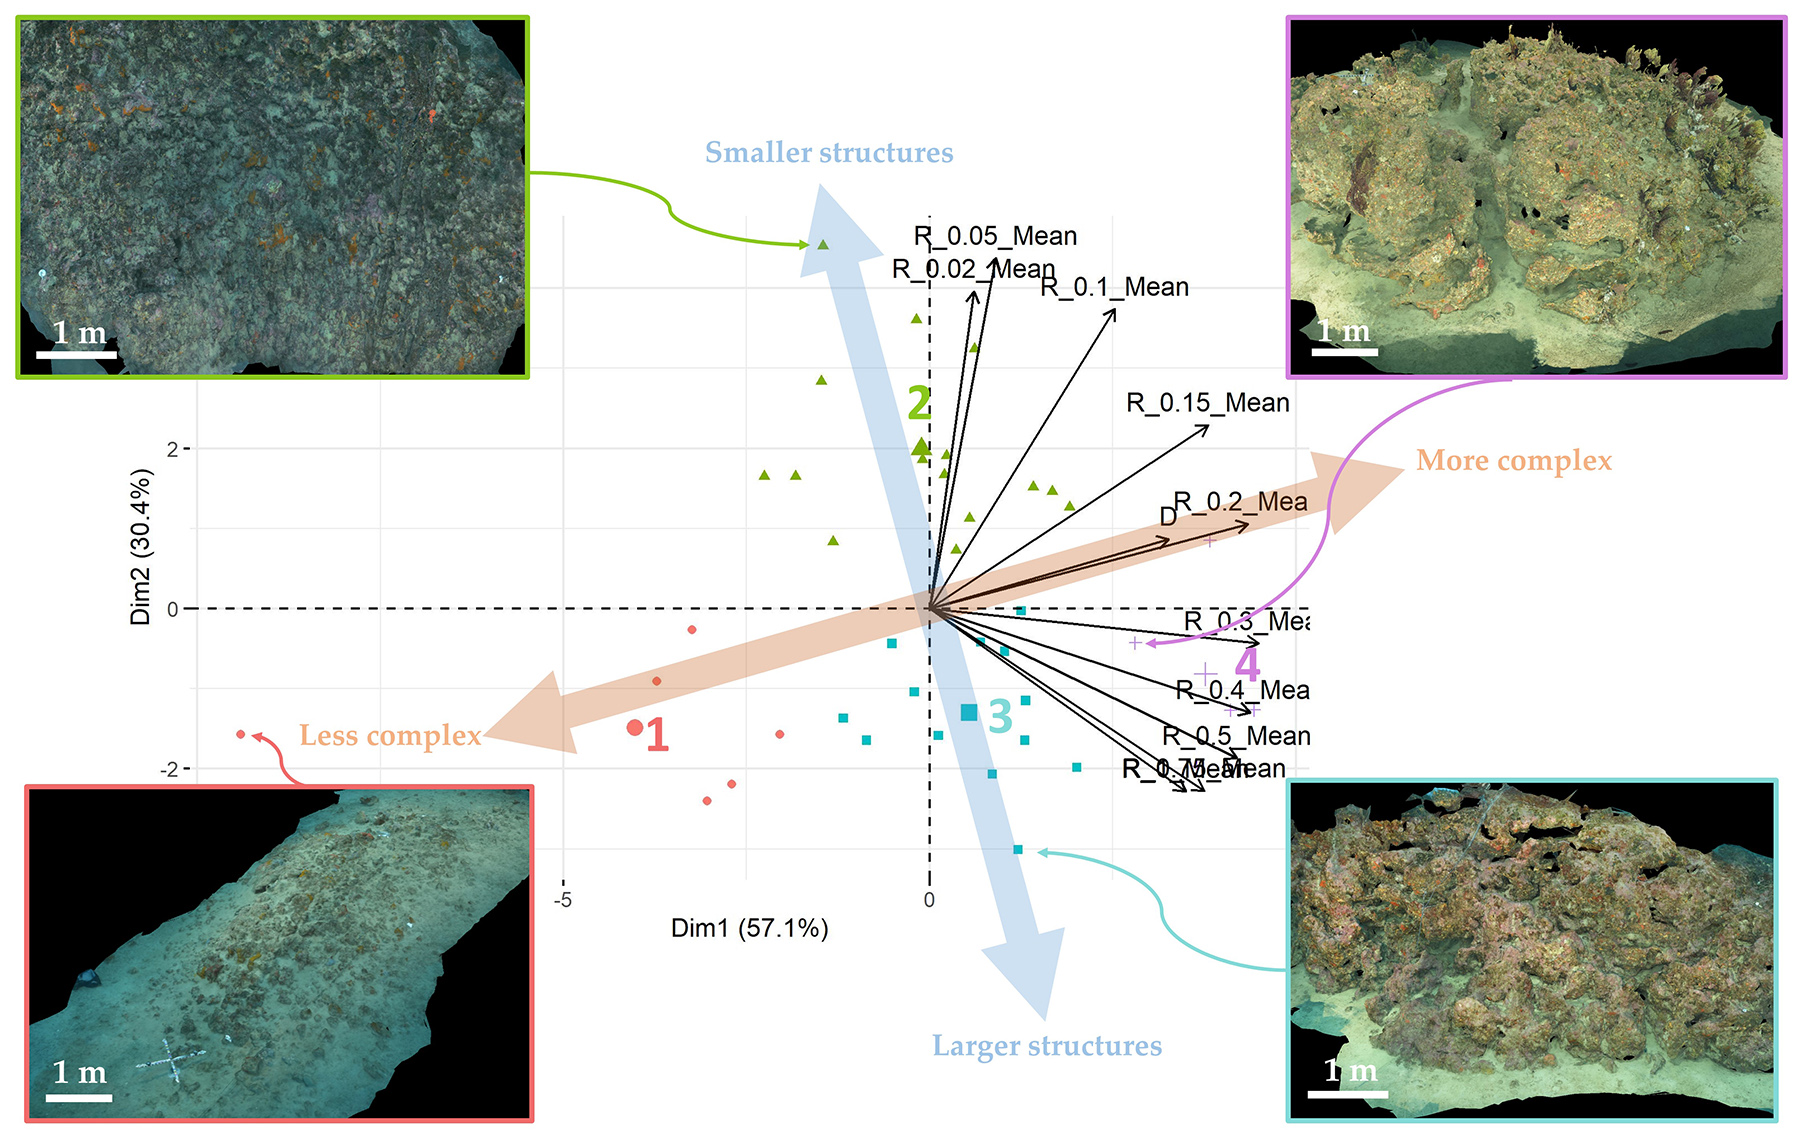
\includegraphics[width=\linewidth,keepaspectratio]{./6_chapitre4/Figure4.3}
		\caption[Biplot of the PCA on structural variables with coralligenous reefs’ morphotypes defined by K-means clustering]{Biplot of the PCA on structural variables with coralligenous reefs’ morphotypes defined by K-means clustering. Black arrows = variables in the first plan: R\_X\_Mean = mean roughness with kernel size X m; D = fractal dimension. Morphotypes: 1 (red) = low complexity; 2 (green) = average complexity / small structures; 3 (cyan) = average complexity / large structures; 4 (purple) = high complexity / large structures. The four images at the corners represent one site example per morphotype.}
	\label{figure4.3}
\end{center}
\end{figure}

F was not significantly different between morphotypes 2 and 3 (\autoref{figure4.4}; t-test; p-value > 0.05) but was significantly different between morphotypes 1 and 2-3 (t-test; p-value < 0.001) and between 2-3 and 4 (t-test; p-value < 0.01). Cavity ranged between 0.6 and 16.4 \% coverage; values were not significantly different across morphotypes 1-2-3 (MWW test; p-value > 0.05) but were significantly higher for morphotype 4 than all others (MWW test; p-value < 0.01).

%%%%%%%%%%%%%%%%%%%%%%%%%%%%%%%%%%%%
%%% Figure 4: Fractal and Cavity %%%
%%%%%%%%%%%%%%%%%%%%%%%%%%%%%%%%%%%%
\begin{figure}[H]
	\begin{center}
	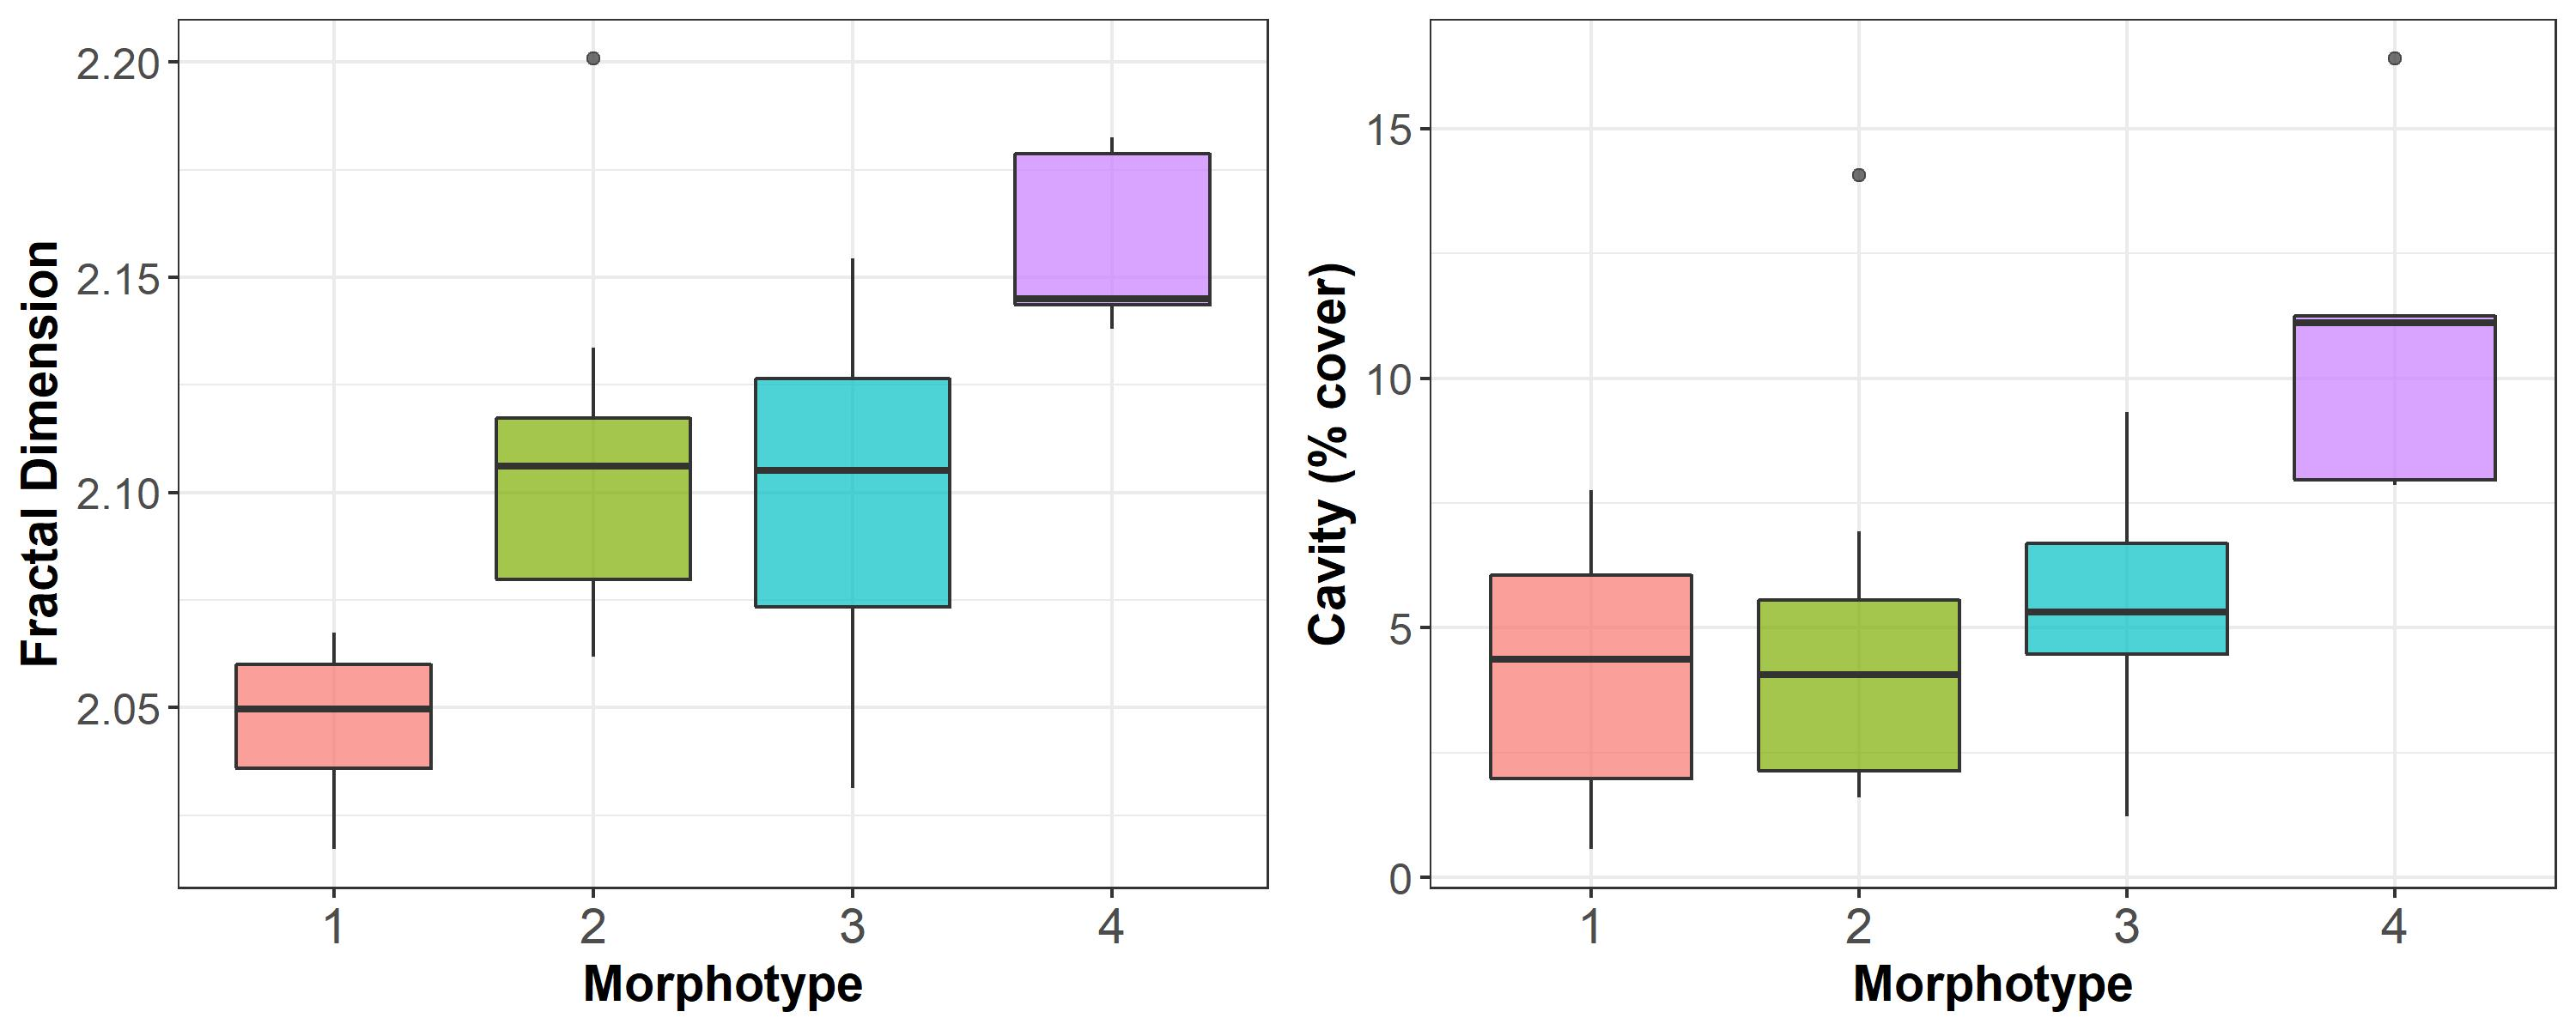
\includegraphics[width=0.7\linewidth,keepaspectratio]{./6_chapitre4/Figure4.4}
		\caption[Fractal Dimension and Cavity (\% cover) in function of the morphotype]{Fractal Dimension and Cavity (\% cover) in function of the morphotype.}
	\label{figure4.4}
\end{center}
\end{figure}


\subsection[Biodiversity and assemblage composition of the morphotypes]{Biodiversity and assemblage composition of the morphotypes}\label{chapitre4_3.2}
TD ranged between 13 and 49 classes, FD ranged between 1.17 and 4.41 across all study sites, and SI ranged between 1.27 and 2.74 (\autoref{figure4.5}). None of the biodiversity indicators were significantly different across morphotypes (MWW; p-value > 0.05), except Shannon Index that was significantly higher for morphotype 2 compared to morphotype 3 (MWW test; p-value < 0.01). 

%%%%%%%%%%%%%%%%%%%%%%%%%%%%%%%
%%% Figure 5: TD, SI and FD %%%
%%%%%%%%%%%%%%%%%%%%%%%%%%%%%%%
\begin{figure}[H]
	\begin{center}
	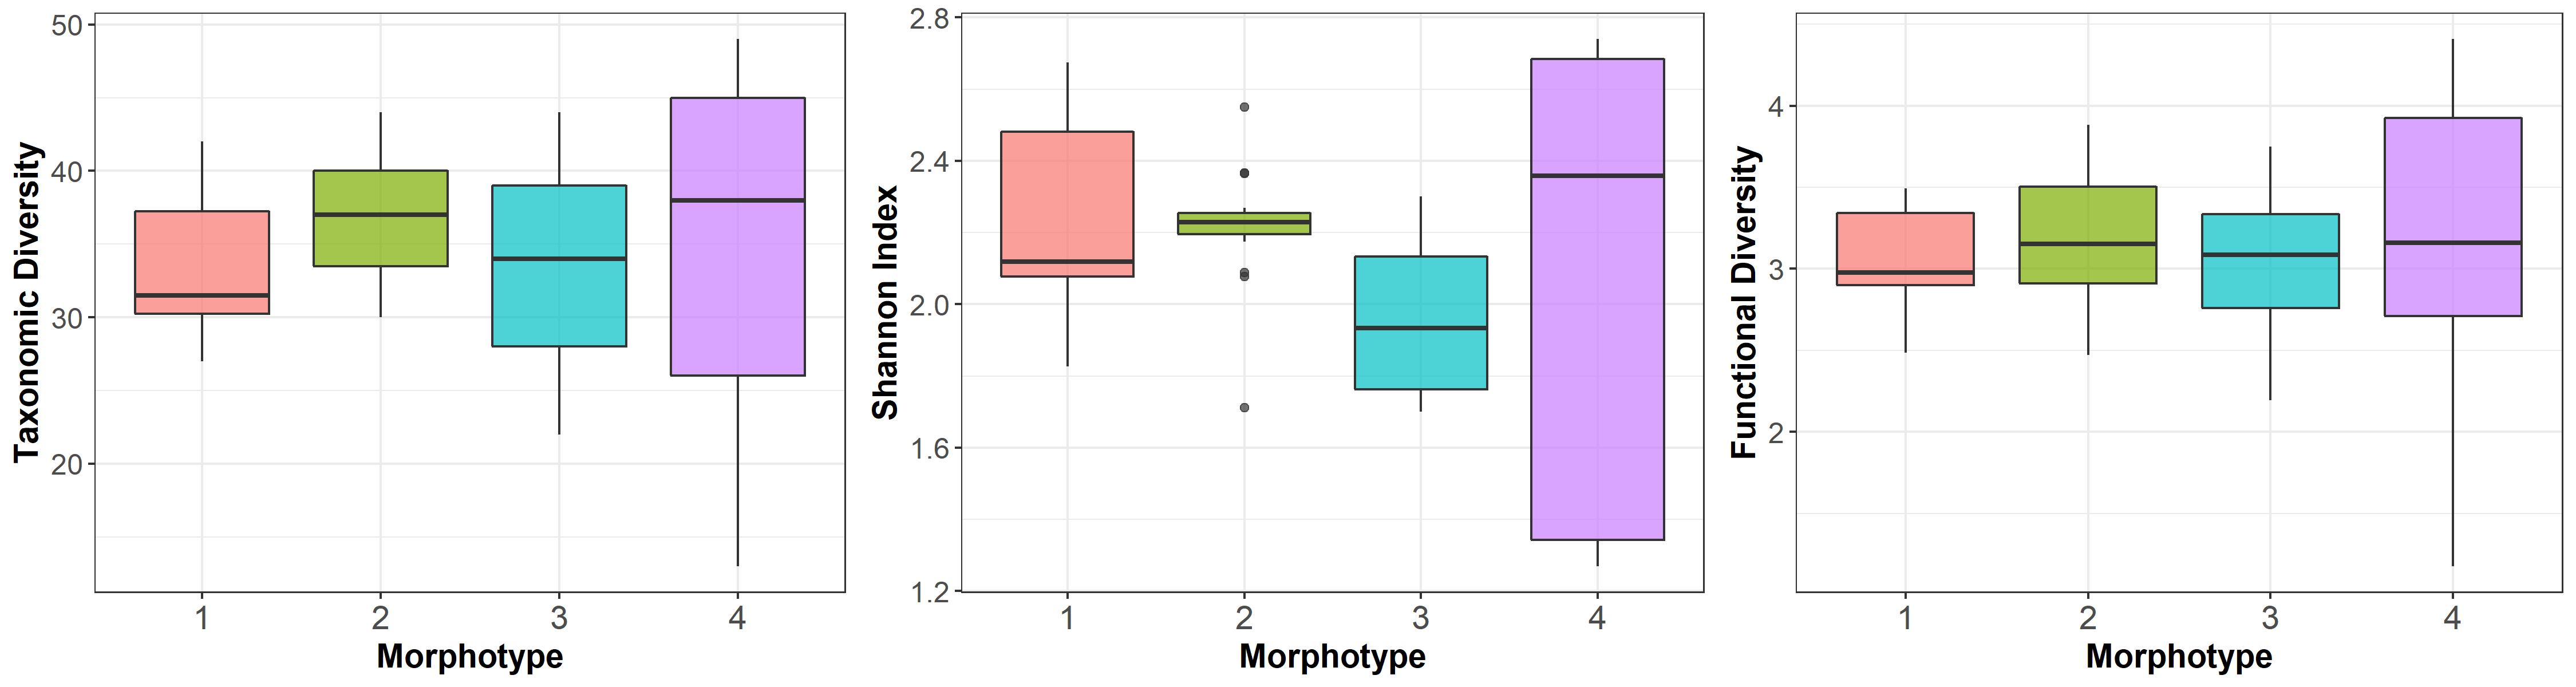
\includegraphics[width=\linewidth,keepaspectratio]{./6_chapitre4/Figure4.5}
		\caption[Taxonomic Diversity, Shannon Index and Functional Diversity, per morphotype]{Taxonomic Diversity, Shannon Index and Functional Diversity, per morphotype.}
	\label{figure4.5}
\end{center}
\end{figure}

CAI ranged between 0.12 and 0.67, and IC ranged between 25.7 and 82.7 (\autoref{figure4.6}). None of the two ecological indicators were significantly different across morphotypes (MWW; p-value > 0.05). CAI and IC were highly correlated (spearman correlation coefficient = 0.77). A LM showed that mean roughness at scales 0.15, 0.4 and 1.0 m significantly explained the SC component of IC, with 27 \% of variance explained. Necrosis relative abundance was higher for morphotypes 1 and 3 than morphotype 4 (MWW; p-value < 0.01).

%%%%%%%%%%%%%%%%%%%%%%%%%%%%%%%%%%%
%%% Figure 6: CAI, IC, Necrosis %%%
%%%%%%%%%%%%%%%%%%%%%%%%%%%%%%%%%%%
\begin{figure}[H]
	\begin{center}
	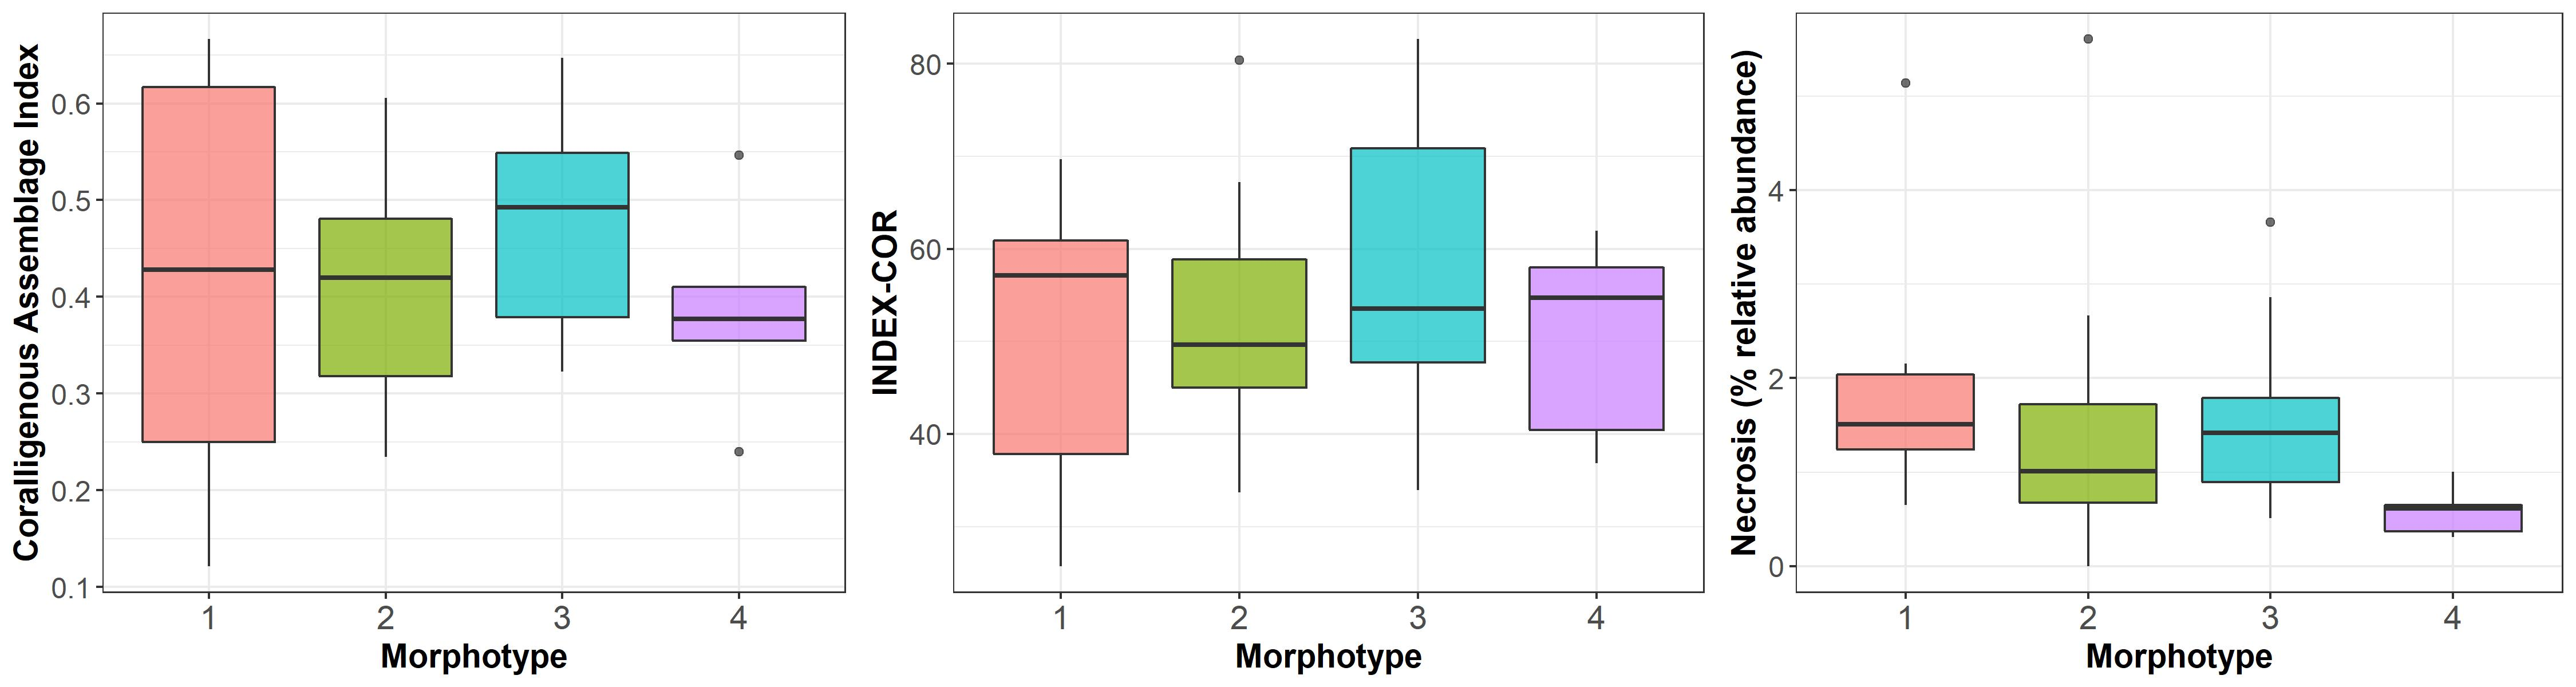
\includegraphics[width=\linewidth,keepaspectratio]{./6_chapitre4/Figure4.6}
		\caption[Coralligenous Assemblage Index, INDEX-COR and necrosis relative abundance, per morphotype]{Coralligenous Assemblage Index, INDEX-COR and necrosis relative abundance, per morphotype.}
	\label{figure4.6}
\end{center}
\end{figure}

PERMANOVA results did not show any significant assemblage composition difference among the four morphotypes (p-value > 0.05), evidenced by the overlaying convex hulls on the nMDS two dimensional plot (\autoref{figure4.7}).

%%%%%%%%%%%%%%%%%%%%%%%%%%%%%%%%%%%%%%%%%%%
%%% Figure 7: nMDS two-dimensional plot %%%
%%%%%%%%%%%%%%%%%%%%%%%%%%%%%%%%%%%%%%%%%%%
\begin{figure}[H]
	\begin{center}
	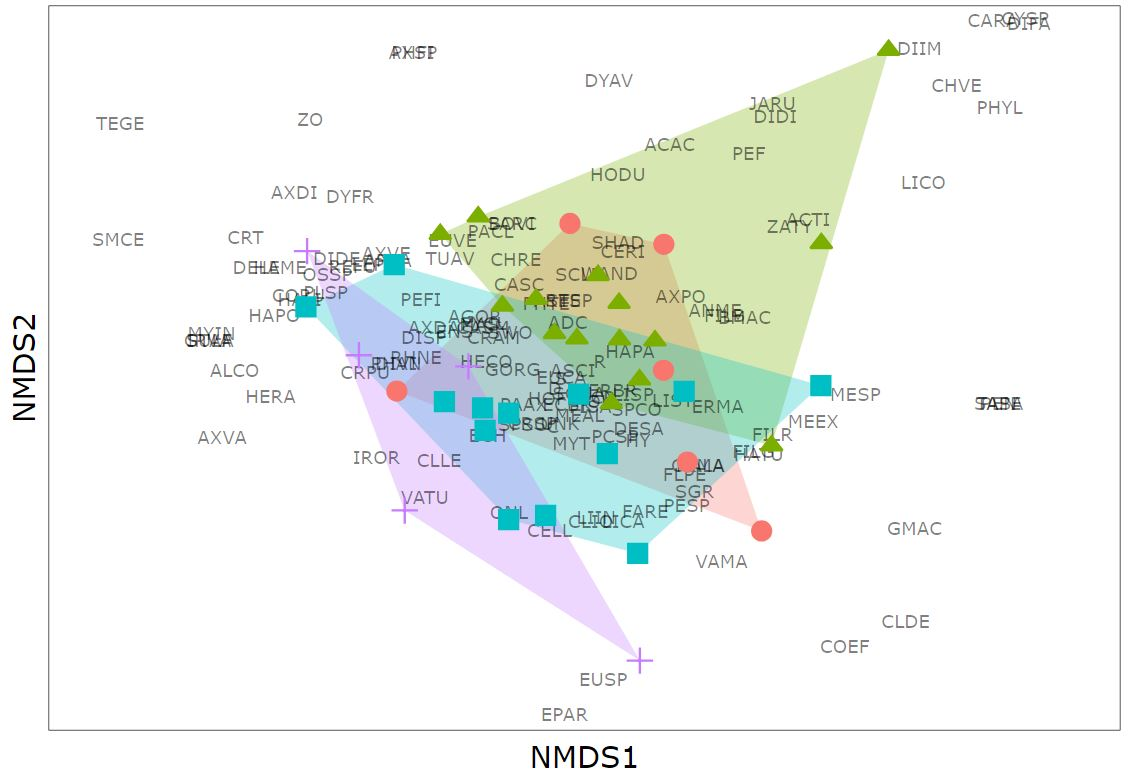
\includegraphics[width=\linewidth,keepaspectratio]{./6_chapitre4/Figure4.7}
		\caption[Two dimensional nMDS ordination of the species abundance data]{Two dimensional nMDS ordination of the species abundance data. Coloured polygons represent the convex hulls of the four morphotypes (morphotype 1 in red, morphotype 2 in green, morphotype 3 in blue and morphotype 4 in purple). Full species names available in \autoref{annexe-species}.}
	\label{figure4.7}
\end{center}
\end{figure}

\subsection{Links between morphotypes and environment}\label{chapitre4_3.3}
All metrics of structural complexity were poorly correlated with environmental variables (spearman correlation coefficient < 0.3). Conversely, none of the environmental variables had a significant effect on the fractal dimension and roughness descriptors (t-test; p-value > 0.05). Environmental variables varied across the morphotypes and depending on the category (\autoref{figure4.8}). Depth was lower for morphotype 2 than 3 (MWW; p-value < 0.05), suspended particulate matter was greater for morphotype 2 than 3 (MWW; p-value < 0.05); N-S current was higher for morphotypes 1 and 4 than 2, and higher for morphotype 1 than 3 (MWW; p-value < 0.05).

%%%%%%%%%%%%%%%%%%%%%%%%%%%%%%%%%%%%%%%%%
%%% Figure 8: Environmental variables %%%
%%%%%%%%%%%%%%%%%%%%%%%%%%%%%%%%%%%%%%%%%
\begin{figure}[H]
	\begin{center}
	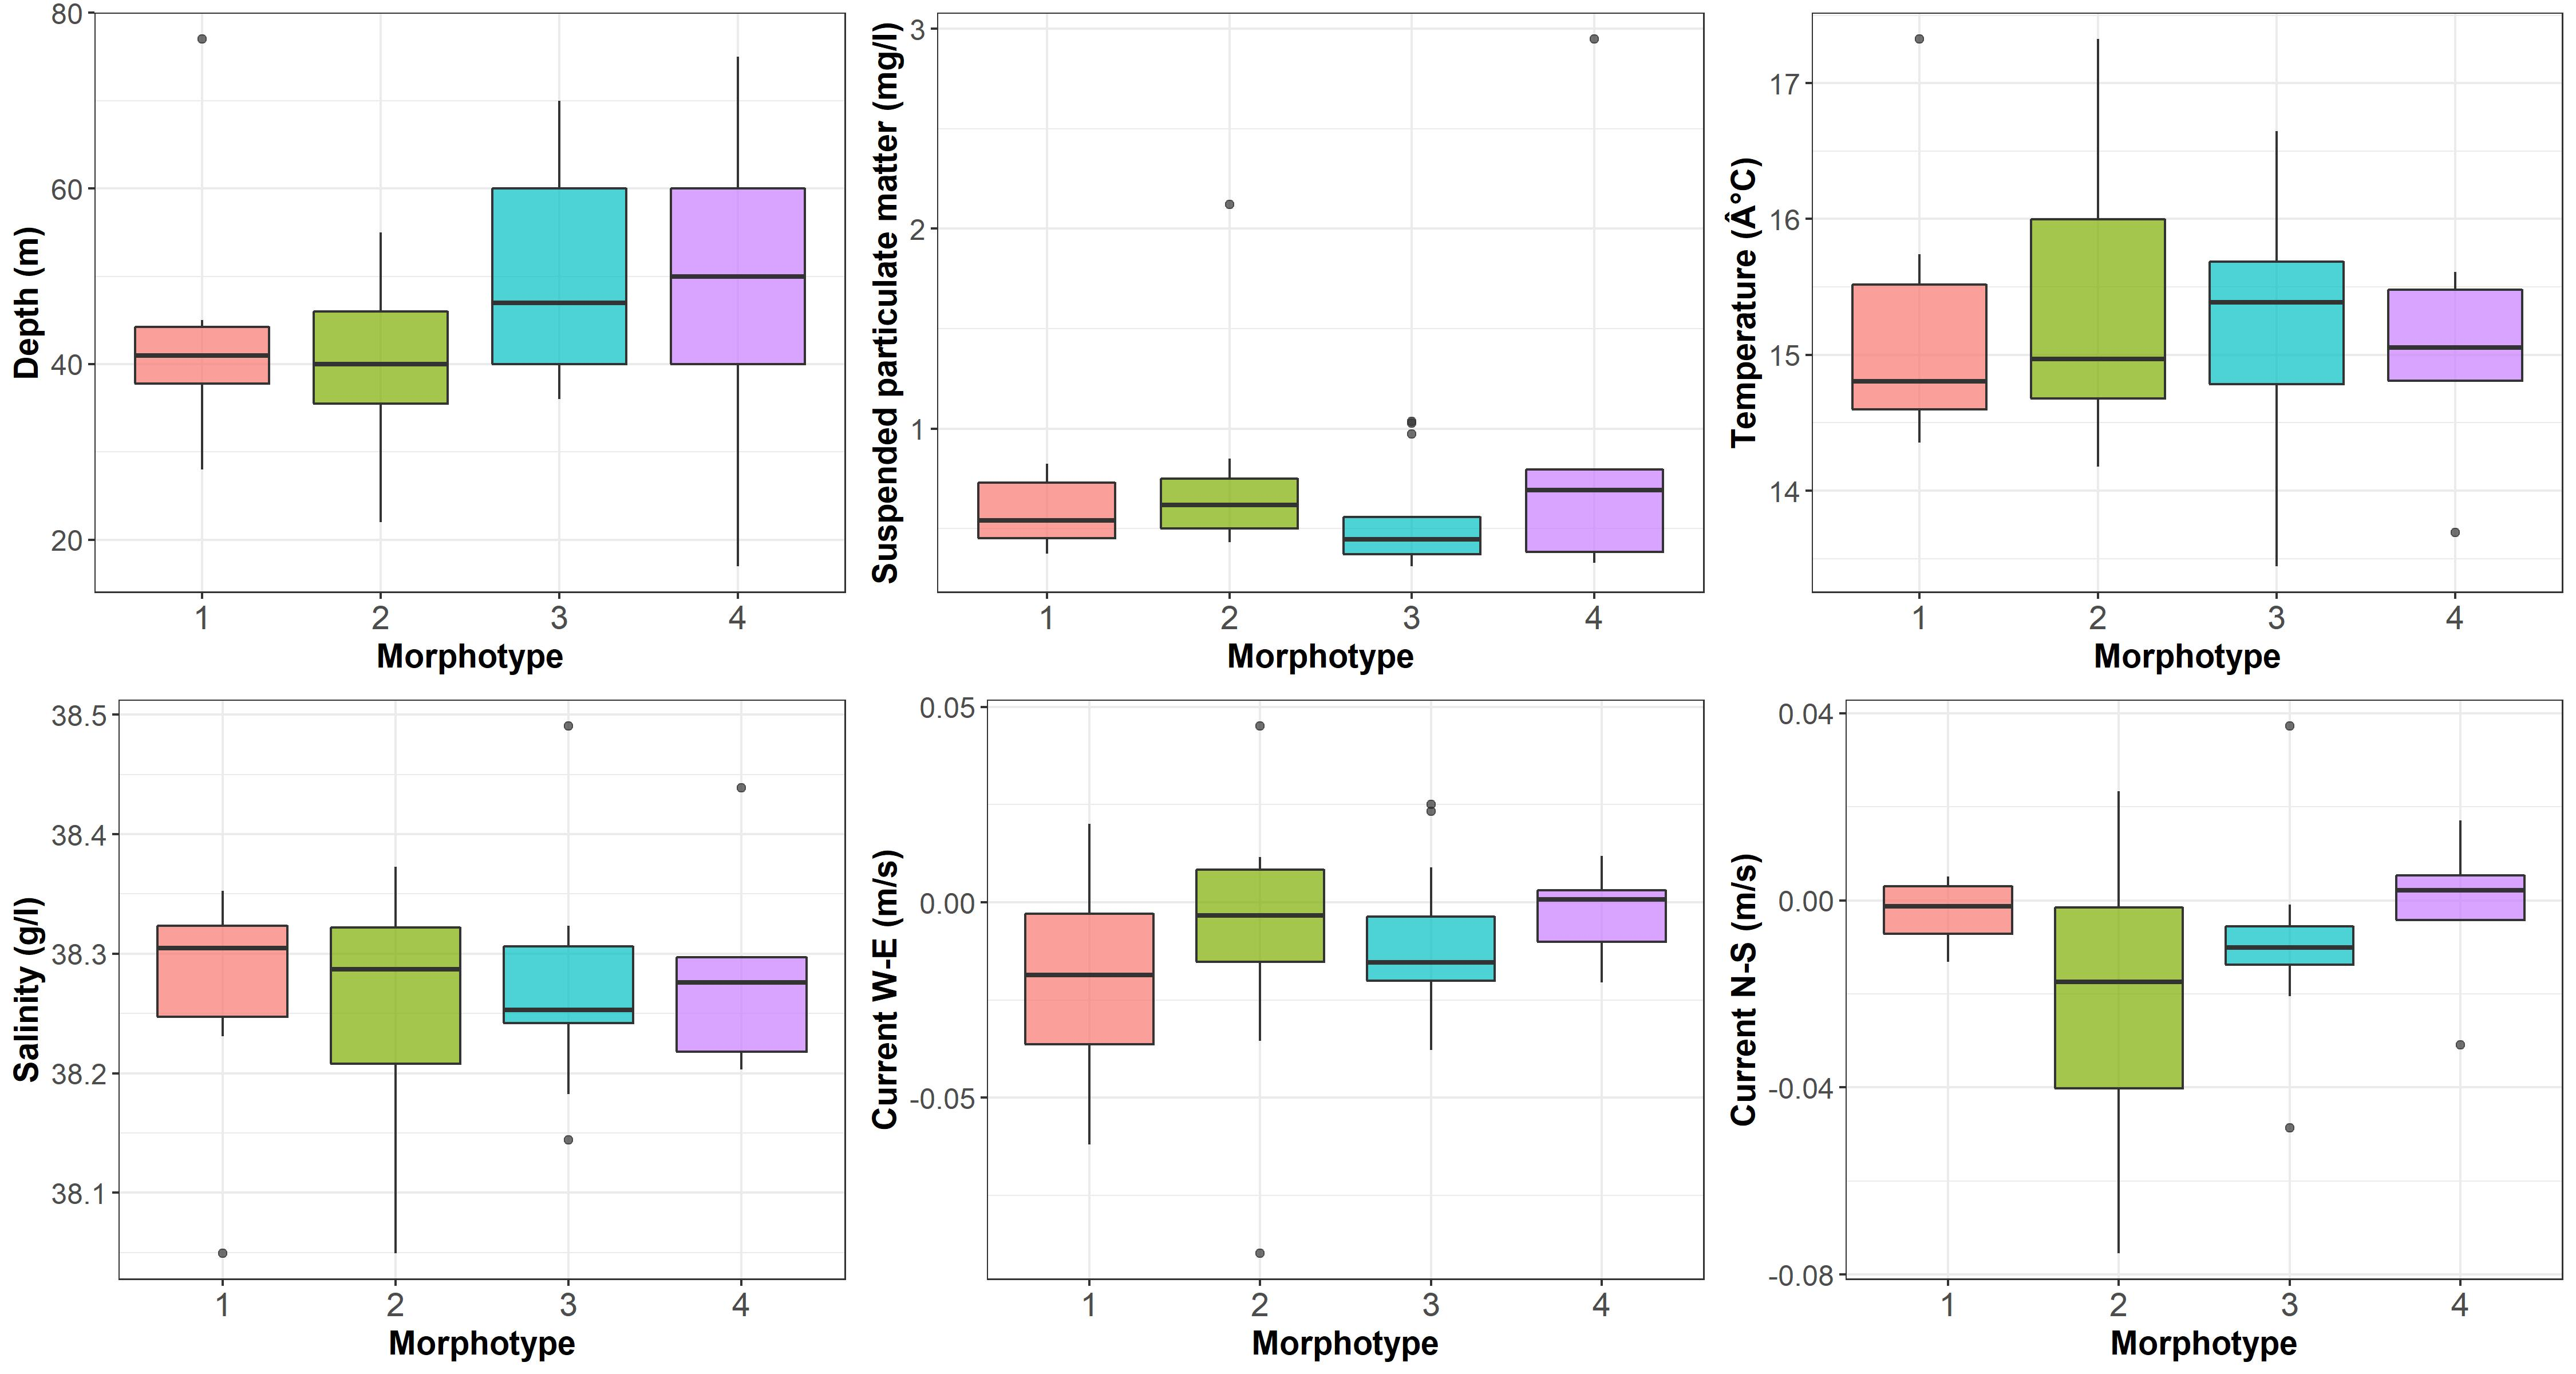
\includegraphics[width=\linewidth,keepaspectratio]{./6_chapitre4/Figure4.8}
		\caption[Distribution of environmental variables per morphotype]{Distribution of environmental variables per morphotype. Values represent means of each variable over the period 2015-01 to 2019-11.}
	\label{figure4.8}
\end{center}
\end{figure}


\section{Discussion}\label{chapitre4_4}

\subsection{On the characterisation of coralligenous reefs’ morphology}\label{chapitre4_4.1}
The 39 study sites used in this first approach to characterise coralligenous reefs’ structure showed a great variety of morphologies, from relatively flat and low complexity sites to boulders with high structural complexity. We defined four different morphotypes of coralligenous reefs based on descriptors of surface roughness at different scales and fractal dimension: low complexity (morphotype 1), average complexity with small or large structures (respectively morphotypes 2 and 3), and high complexity with large structures (mophotype 4). Significantly more cavities were observed for morphotype 4 compared to the three others (MWW; p-value < 0.01), which is consistent with the higher values of mean roughness at large scales (> 0.3 m) for this morphotype. Morphotypes 2 and 3 were about the same level of fractal dimension, but morphotype 3 was characterised by larger structures (\autoref{figure4.3}). These four morphotypes were then used to whether the structure determines the ecological assemblages and whether it is influenced by the local environmental conditions.

\subsection{Ecological and environmental implications}\label{chapitre4_4.2}
We did not detect any significant difference of diversity metrics across the four morphotypes, with the exception of SI that was higher for morphotype 2 than 3 (MWW test; p-value < 0.01), suggesting that abundances in the assemblages of morphotype 2 were more evenly distributed than for morphotype 3. These findings contrast with recent studies that concluded, in the case of coral reefs, that the different facets of the coral diversity were key drivers of the structural complexity \citep{darling_relationships_2017, price_using_2019}. Interestingly, it seems that the variances of biodiversity and ecological indices among morphotypes were opposed: if TD, SI and FD had the greatest variance for morphotype 4, the three other morphotypes having similar variances, CAI and IC showed the lowest variance for morphotype 4 and the highest for morphotype 1. In essence, this suggests that the composition of assemblages for morphotypes with greater structural complexity had similar ecological status, although they included a range of different compositions. However, the PERMANOVA showed no significant differences in species composition among the four morphotypes, as suggested by the overlaying convex hulls on the nMDS two dimensional plot (\autoref{figure4.7}). The lower level of necrosis observed for morphotype 4 might be due to the slightly higher level of sponges for this morphotype (species labels of the upper left corner of \autoref{figure4.7}). Indeed, few necroses are observed for this major categoriy.

We also explored the links between the morphotypes and some environmental variables, extracted from Previmer model and averaged over five years. Although some differences were significant across morphotypes, we did not observe any true pattern that could explain the structural differences, notably environmental conditions that could favour the growth of some particular organisms contributing to the structural complexity of the reefs. However, the environmental variables corresponded to modelled conditions over a short period of time (2015-2019) compared to the time required for the growth and building of these reefs (hundreds to thousands of years \citep{sartoretto_age_1996}). If some environmental conditions such as temperature probably influence the growth and composition of coralligenous assemblages, and therefore the structure of the reefs, we could not assess their effect at the entire reefs lifetime. Furthermore, values were extracted from the relatively coarse 10 $\times$ 10 km grid of Previmer model with 60 depth levels per cell, which does not really correspond to the highly complex and variable local conditions met according to the depth and local site configuration \citep{kipson_rapid_2011, willis_habitat_2005}.

\subsection{Possible issues and perspectives}\label{chapitre4_4.3}
Although some slight differences were observed across morphotypes, results did not show any true pattern, notably the expected higher diversity and ecological quality of more complex reefs such as for coral reefs \citep{darling_relationships_2017, price_using_2019}. We propose several hypotheses that could explain these results and should be investigated in future work. First, although similar in terms of biodiversity and production, coralligenous reefs have different growth and mortality dynamics than coral reefs. Notably, coralligenous reefs lie in average much deeper down the sea surface than most studied coral reefs; consequently, they are far less sensitive to wave exposure, and a dead part of a reef will take a long time to be physically or biologically altered / recolonised. In opposition, bleaching events in tropical reefs are rapidly followed by the colonisation by macroalgae or broken down by the movement of waves \citep{graham_predicting_2015}. This suggests that a major part of the current structure measured on the 3D models could be the reflect of the reefs’ history more than its current composition and state. One of the study sites in particular (Centrale) was highly complex in structure but showed the lowest diversity and ecological status because of its current high mud coverage., due to coastal anthropogenic sediment loads \citep{airoldi_effects_2003, ballesteros_mediterranean_2006}. If this hypothesis was confirmed, structural complexity of coralligenous reefs could be seen as the ecological potential of the reef, and linking with the current assemblage composition would highlight its true ecological status. Conversely, metrics showing low biodiversity / functioning and low structural complexity could be the reflect of a “young” reef in development.

Second, our results might also be due to our sampling procedure. Indeed, contrary to some studies were 3D models were exhaustively labelled (all visible individuals were tagged and labelled in 3D) \citep{price_using_2019}, our data was composed of 3D reefs with corresponding photo quadrats randomly taken over the reef. This sampling procedure can have important drawbacks on the results, as in some cases the photo quadrats can correspond to a limited part of the 3D model, which then captures structural noise without the corresponding ecological data. Also, reconstruction artefacts can underestimate some of the structural descriptors, such as gorgonians that are sometimes not well reconstructed in the case of strong currents or very large individuals, due to their soft skeleton.

Finally, coralligenous reefs are highly complex assemblages whose composition is the result of the interaction of multiple ecological and environmental factors through time. This complexity produces a very high composition variability across reefs, even locally within a reef, which are not well understood yet. Such variability probably requires a much larger sampling effort to be able to capture individual effects of each factor, among which the reef structure. 

If our data did not allow to detect any strong correlations between structural metrics and the composition of today’s living organisms on the reef, the structure has been showed to play an important role in fish diversity and biomass on coral reefs \citep{darling_relationships_2017, graham_importance_2013, price_using_2019, willis_habitat_2005}. As their tropical relatives, coralligenous reefs host an abundant and diverse mobile fauna \citep{ballesteros_mediterranean_2006} and it is more than probable that structure also influences the abundance and diversity of benthic and demersal fishes in the case of coralligenous reefs.


\section{Conclusion}\label{chapitre4_5}
This study represents a first approach towards the characterisation of coralligenous reefs’ structural complexity and the relationships with the quality and diversity of the assemblages. We used 3D photogrammetric models to define four morphotypes based on multiple structural indices and assessed assemblage differences among these. If our data did not show any clear relationships between the structure and the diversity of coralligenous assemblages, the amount of available data in relation with the complexity of these links does not allow any conclusion. Data should ideally include annotations directly on the 3D reconstruction, with the help of deep learning to massively annotate the 3D models. This would allow to work at different scales and link local diversity with local structure. Future work should also consider the links between structural complexity and fish diversity and abundance, with the use of 2D acoustics or video counting.

\medskip

\noindent\textbf{Acknowledgments:} We thank Kyle Zawada for sharing his R custom version of the box-counting algorithm for calculating the fractal dimension of the reefs. We also thank Juliette Langlois and Nicolas Mouquet for their help with the functional traits database, and François Guilhaumon for sharing the R script for computing the functional diversity. The acquisition of the data was possible thanks to the logistic support of Andromède Océanologie and the French Water Agency during the annual fieldwork campaigns of RECOR monitoring network (http://www.medtrix.fr).